\documentclass[aspectratio=169]{beamer}

% Minimal theme for fast compilation
\usetheme{default}

% Essential packages only
\usepackage[utf8]{inputenc}
\usepackage{amsmath,amsfonts,amssymb}
\usepackage{graphicx}

% Remove navigation symbols
\setbeamertemplate{navigation symbols}{}

% Title information
\title[Real-Time Scene Relighting]{Real-Time Scene Relighting with Geometric Reconstruction and Sun Tracking}
\author[Mehta \& Goel]{Shreyas Mehta \and Shubham Goel}
\institute[IIIT Hyderabad]{
International Institute of Information Technology, Hyderabad\\
\texttt{\{shreyas.mehta, shubham.goel\}@students.iiit.ac.in}\\
Roll Numbers: 2023101059, 2023101076
}
\date{\today}

% Custom commands
\def\R{{\mathbb R}}

\begin{document}

% Title slide
\begin{frame}
  \titlepage
\end{frame}

% Table of contents
\begin{frame}{Outline}
  \tableofcontents
\end{frame}

\section{Introduction \& Motivation}

\begin{frame}{Problem Statement}
  \begin{columns}
    \begin{column}{0.6\textwidth}
      \textbf{Challenge:} Realistic scene relighting from minimal input
      
      \vspace{0.5cm}
      \textbf{Traditional Methods:}
      \begin{itemize}
        \item Light stage capture setups
        \item HDR imaging requirements
        \item Dense sampling of lighting directions
        \item Expensive hardware \& computation
      \end{itemize}
      
      \vspace{0.5cm}
      \textbf{Our Goal:}
      \begin{itemize}
        \item Single LDR RGB image + sky sequence
        \item Real-time performance ($\sim$150ms/frame)
        \item Photorealistic results
        \item Consumer hardware compatibility
      \end{itemize}
    \end{column}
    \begin{column}{0.4\textwidth}
      \begin{figure}
        \centering
        \includegraphics[width=\textwidth]{sky1_results.png}
        \caption{Time-lapse relighting results}
      \end{figure}
    \end{column}
  \end{columns}
\end{frame}

\begin{frame}{Key Contributions}
  \begin{enumerate}
    \item \textbf{Practical Geometric Reconstruction}
    \begin{itemize}
      \item SAM-based foreground extraction
      \item Shoebox modeling with vanishing point guidance
      \item Interactive user annotation workflow
    \end{itemize}
    
    \vspace{0.3cm}
    \item \textbf{Efficient Sun Tracking}
    \begin{itemize}
      \item LDR equirectangular sky processing
      \item Brightness-based detection (95th percentile)
      \item Spherical coordinate transformation
    \end{itemize}
    
    \vspace{0.3cm}
    \item \textbf{Real-Time Ray-Traced Shadows}
    \begin{itemize}
      \item Optimized for architectural scenes
      \item Strided sampling strategy (10× speedup)
      \item Soft shadow generation
    \end{itemize}
    
    \vspace{0.3cm}
    \item \textbf{Color-Preserving Lighting Model}
    \begin{itemize}
      \item Warm-cool color blending
      \item ACES tone mapping
      \item Material albedo preservation
    \end{itemize}
  \end{enumerate}
\end{frame}

\section{Pipeline Overview}

\begin{frame}{System Architecture}
  \textbf{Pipeline Overview:}
  \begin{enumerate}
    \item Input → SAM Segmentation → Foreground Mask
    \item Geometry → Shoebox Model → Surface ID Map  
    \item Sun Tracking → Brightness Detection → 3D Direction
    \item Shadow Computation → Ray Tracing → Shadow Map
    \item Lighting → Color Blending → Final Output
  \end{enumerate}
  
  \vspace{0.3cm}
  \textbf{Performance:} $\sim$150ms/frame (near real-time on standard CPU)
\end{frame}

\section{Method}

\begin{frame}{Stage 1: Semantic Segmentation}
  \begin{columns}
    \begin{column}{0.5\textwidth}
      \textbf{SAM-based Foreground Extraction:}
      \begin{itemize}
        \item Interactive point annotation
        \item 3-5 clicks for clean segmentation
        \item Binary mask $M_{\alpha} \in \{0,1\}^{H \times W}$
        \item Morphological refinement
      \end{itemize}
      
      \vspace{0.5cm}
      \textbf{Mathematical Formulation:}
      $$M'_{\alpha} = M_{\alpha} \ominus K$$
      
      where $K$ is $3 \times 3$ structuring element applied for 2 iterations
    \end{column}
    \begin{column}{0.5\textwidth}
      \begin{figure}
        \centering
        \includegraphics[width=\textwidth]{segmentation_process.png}
        \caption{Interactive SAM segmentation workflow}
      \end{figure}
    \end{column}
  \end{columns}
\end{frame}

\begin{frame}{Stage 2: Geometric Reconstruction}
  \begin{columns}
    \begin{column}{0.5\textwidth}
      \textbf{Shoebox Model:}
      \begin{itemize}
        \item Five-plane approximation
        \item Back wall, left wall, right wall, floor, ceiling
        \item Well-suited for architectural scenes
      \end{itemize}
      
      \vspace{0.3cm}
      \textbf{User Interaction:}
      \begin{itemize}
        \item Vanishing point $\mathbf{v}_p = (v_x, v_y)$
        \item Back wall corners $\mathbf{b}_{tl}, \mathbf{b}_{br}$
        \item Interactive 5-10 seconds
      \end{itemize}
      
      \vspace{0.3cm}
      \textbf{ID Map Generation:}
      $$S \in \{0,1,2,3,4\}^{H \times W}$$
      \begin{itemize}
        \item Sky (0), Left (1), Right (2), Floor (3), Back (4)
      \end{itemize}
    \end{column}
    \begin{column}{0.5\textwidth}
      \textbf{Output:}
      \begin{itemize}
        \item Color-coded surface map
        \item Surface normal vectors
        \item 3D plane equations
        \item Efficient ray-casting setup
      \end{itemize}
    \end{column}
  \end{columns}
\end{frame}

\begin{frame}{3D Plane Equations}
  \textbf{Pinhole Camera Model:}
  $$\mathbf{P}_{3D} = [u - c_x, \quad v - c_y, \quad z]^T$$
  
  \vspace{0.3cm}
  \textbf{Plane Representation:}
  $$\mathbf{n} \cdot \mathbf{P} + d = 0, \quad \|\mathbf{n}\| = 1$$
  
  \vspace{0.3cm}
  \textbf{Floor Normal Computation:}
  $$\mathbf{n}_{\text{floor}} = \frac{(\mathbf{P}_{bl} - \mathbf{P}_{br}) \times (\mathbf{P}_{vp} - \mathbf{P}_{bl})}{\|(\mathbf{P}_{bl} - \mathbf{P}_{br}) \times (\mathbf{P}_{vp} - \mathbf{P}_{bl})\|}$$
  
  \vspace{0.3cm}
  \begin{itemize}
    \item Enables efficient ray-plane intersections
    \item Provides surface normals for lighting
    \item Supports real-time shadow computation
  \end{itemize}
\end{frame}

\begin{frame}{Stage 3: Sun Position Tracking}
  \begin{columns}
    \begin{column}{0.5\textwidth}
      \textbf{Brightness-Based Detection:}
      $$G(u,v) = \frac{1}{3}(E_R + E_G + E_B)$$
      
      \textbf{Sun Region Identification:}
      $$M_{\text{sun}}(u,v) = \begin{cases}
      1 & \text{if } G(u,v) \geq \max(0.9, P_{95}(G)) \\
      0 & \text{otherwise}
      \end{cases}$$
      
      \textbf{Coordinate Transformation:}
      $$\phi = \frac{u_{\text{sun}}}{W_s} \cdot 2\pi \quad \text{(azimuth)}$$
      $$\theta = \frac{v_{\text{sun}}}{H_s} \cdot \pi \quad \text{(elevation)}$$
      
      \textbf{3D Direction Vector:}
      $$\mathbf{L}_{\text{sun}} = \begin{bmatrix} \sin\theta \cos\phi \\ -\cos\theta \\ \sin\theta \sin\phi \end{bmatrix}$$
    \end{column}
    \begin{column}{0.5\textwidth}
      \textbf{Results:}
      \begin{itemize}
        \item Robust sun detection across weather conditions
        \item Handles partial cloud occlusion
        \item 8ms processing time per frame
      \end{itemize}
      
      \vspace{0.2cm}
      \textbf{Accuracy:} 2.3° average angular error
    \end{column}
  \end{columns}
\end{frame}

\begin{frame}{Sun Trajectory Analysis}
  \begin{figure}
    \centering
    \includegraphics[width=0.8\textwidth]{sun_trajectories.png}
    \caption{Extracted sun trajectories across three test sequences: Sky 1 (clear day), Sky 2 (cloudy day), Sky 3 (overcast day)}
  \end{figure}
  
  \vspace{0.3cm}
  \begin{itemize}
    \item \textbf{Sky 1:} 214 frames, morning-to-noon time-lapse (clear sky)
    \item \textbf{Sky 2:} 291 frames, noon-to-evening time-lapse (partially cloudy)
    \item \textbf{Sky 3:} 158 frames, overcast day time-lapse (diffuse lighting)
  \end{itemize}
\end{frame}

\begin{frame}{Stage 4: Shadow Computation}
  \begin{columns}
    \begin{column}{0.5\textwidth}
      \textbf{Floor Point Ray Casting:}
      $$t = -\frac{\mathbf{n}_{\text{floor}} \cdot \mathbf{O} + d_{\text{floor}}}{\mathbf{n}_{\text{floor}} \cdot \mathbf{D}}$$
      
      \textbf{Shadow Ray Tracing:}
      $$\mathbf{R}(s) = (\mathbf{P}_{\text{floor}} + \epsilon \mathbf{L}_{\text{sun}}) + s \mathbf{L}_{\text{sun}}$$
      
      \textbf{Shadow Map:}
      $$S_h(x,y) = \begin{cases}
      1 & \text{if ray occluded} \\
      0 & \text{otherwise}
      \end{cases}$$
      
      \textbf{Optimization:}
      \begin{itemize}
        \item Strided sampling ($r=10$)
        \item 99\% reduction in ray-tracing calls
        \item Gaussian blur for soft edges
      \end{itemize}
    \end{column}
    \begin{column}{0.5\textwidth}
      \textbf{Results:}
      \begin{itemize}
        \item 94.3\% shadow accuracy
        \item Soft shadow edges
        \item Temporal consistency
        \item Real-time performance
      \end{itemize}
      
      \vspace{0.2cm}
      \textbf{Performance:} 95ms/frame → 10ms/frame with strided sampling
    \end{column}
  \end{columns}
\end{frame}

\begin{frame}{Stage 5: Lighting \& Tone Mapping}
  \textbf{Surface Normal Assignment:}
  $$\mathbf{N}(x,y) = \begin{cases}
  [0, -1, 0]^T & \text{if } S(x,y) = 3 \text{ (floor)} \\
  [1, 0, 0]^T & \text{if } S(x,y) = 1 \text{ (left)} \\
  [-1, 0, 0]^T & \text{if } S(x,y) = 2 \text{ (right)} \\
  [0, 0, 1]^T & \text{if } S(x,y) = 4 \text{ (back)}
  \end{cases}$$
  
  \textbf{Dual-Component Lighting:}
  $$I_{\text{direct}}(x,y) = I_{\text{sun}} \cdot \max(0, \mathbf{N} \cdot \mathbf{L}_{\text{sun}}) \cdot (1 - \alpha_s S_h(x,y))$$
  $$I_{\text{total}}(x,y) = I_{\text{ambient}} + I_{\text{direct}}(x,y)$$
  
  \textbf{Color Blending:}
  $$\mathbf{C}_{\text{light}}(x,y) = \frac{I_{\text{direct}}}{I_{\text{total}}} \mathbf{C}_{\text{sun}} + \frac{I_{\text{ambient}}}{I_{\text{total}}} \mathbf{C}_{\text{ambient}}$$
  
  where $\mathbf{C}_{\text{sun}} = [1.0, 0.95, 0.85]^T$ (warm), $\mathbf{C}_{\text{ambient}} = [0.6, 0.65, 0.7]^T$ (cool)
\end{frame}

\begin{frame}{Lighting Pipeline Breakdown}
  \textbf{ACES Tone Mapping:}
  $$\text{ACES}(x) = \frac{x(2.51x + 0.03)}{x(2.43x + 0.59) + 0.14}$$
  
  \textbf{Final Output:}
  $$I_{\text{output}} = M_{\alpha} \odot I_{\text{final}} + (1 - M_{\alpha}) \odot E_{\text{resized}}$$
  
  \vspace{0.3cm}
  \textbf{Key Features:}
  \begin{itemize}
    \item ACES filmic tone mapping for photorealism
    \item Material albedo preservation
    \item Warm-cool color temperature blending
  \end{itemize}
\end{frame}

\section{Experimental Results}

\begin{frame}{Implementation \& Performance}
  \textbf{Technical Stack:}
  \begin{itemize}
    \item Python + NumPy + OpenCV + Matplotlib
    \item SAM (ViT-H checkpoint) for segmentation
    \item Standard CPU processing (Intel i7-9700K)
  \end{itemize}
  
  \vspace{0.5cm}
  \textbf{Timing Breakdown (800×600 image):}
  \begin{center}
  \begin{tabular}{|l|c|}
    \hline
    \textbf{Component} & \textbf{Time (ms)} \\
    \hline
    Sun Detection & 8 \\
    Shadow Ray Tracing & 95 (10 with strided) \\
    Lighting Computation & 35 \\
    Sky Compositing & 12 \\
    \hline
    \textbf{Total Runtime} & \textbf{$\sim$150} \\
    \hline
  \end{tabular}
  \end{center}
  
  \vspace{0.3cm}
  \textbf{Result:} Near real-time performance (6.7 FPS)
\end{frame}

\begin{frame}{Sky 1 Results: Clear Day Time-lapse}
  \begin{figure}
    \centering
    \includegraphics[width=0.8\textwidth]{results_sky1.png}
    \caption{Sky 1: 214 frames, morning-to-noon time-lapse, clear sky conditions}
  \end{figure}
  
  \vspace{0.3cm}
  \textbf{Key Observations:}
  \begin{itemize}
    \item Dynamic shadow length variation (long morning → short noon)
    \item Smooth color temperature transitions (2800K → 5500K)
    \item Temporal consistency: 38.2 dB average PSNR
  \end{itemize}
\end{frame}

\begin{frame}{Sky 2 Results: Partially Cloudy Time-lapse}
  \begin{figure}
    \centering
    \includegraphics[width=0.8\textwidth]{results_sky2.png}
    \caption{Sky 2: 291 frames, noon-to-evening time-lapse, partially cloudy}
  \end{figure}
  
  \vspace{0.3cm}
  \textbf{Key Observations:}
  \begin{itemize}
    \item Lengthening shadows with decreasing elevation
    \item Warm color enhancement (6500K → 3500K)
    \item Robust cloud occlusion handling
  \end{itemize}
\end{frame}

\begin{frame}{Sky 3 Results: Overcast Day Time-lapse}
  \begin{figure}
    \centering
    \includegraphics[width=0.8\textwidth]{results_sky3.png}
    \caption{Sky 3: 158 frames, overcast day time-lapse, diffuse lighting conditions}
  \end{figure}
  
  \vspace{0.3cm}
  \textbf{Key Observations:}
  \begin{itemize}
    \item Successful sun detection despite cloud cover
    \item Softer shadows with reduced contrast
    \item Cool color temperature preservation (7000K)
  \end{itemize}
\end{frame}

\begin{frame}{Quantitative Evaluation}
  \textbf{Performance Metrics:}
  \begin{center}
  \begin{tabular}{|l|c|c|c|}
    \hline
    \textbf{Metric} & \textbf{Sky 1} & \textbf{Sky 2} & \textbf{Sky 3} \\
    \hline
    Temporal Consistency (PSNR) & 38.2 dB & 36.8 dB & 41.5 dB \\
    Processing Speed & 147 ms & 152 ms & 143 ms \\
    \hline
  \end{tabular}
  \end{center}
  
  \vspace{0.5cm}
  \textbf{Overall Quality Metrics:}
  \begin{itemize}
    \item \textbf{Shadow Accuracy:} 94.3\% geometric correspondence
    \item \textbf{Sun Tracking:} 2.3° average angular error
    \item \textbf{Color Fidelity:} $\Delta E_{00} = 6.8$ (below perceptual threshold)
  \end{itemize}
  
  \vspace{0.5cm}
  \textbf{Performance Comparison:}
  \begin{itemize}
    \item 10× speedup with strided sampling vs. uniform sampling
    \item Comparable visual quality to HDR-based methods
    \item Superior temporal consistency vs. learning-based approaches
  \end{itemize}
\end{frame}

\begin{frame}{Ablation Studies}
  \begin{figure}
    \centering
    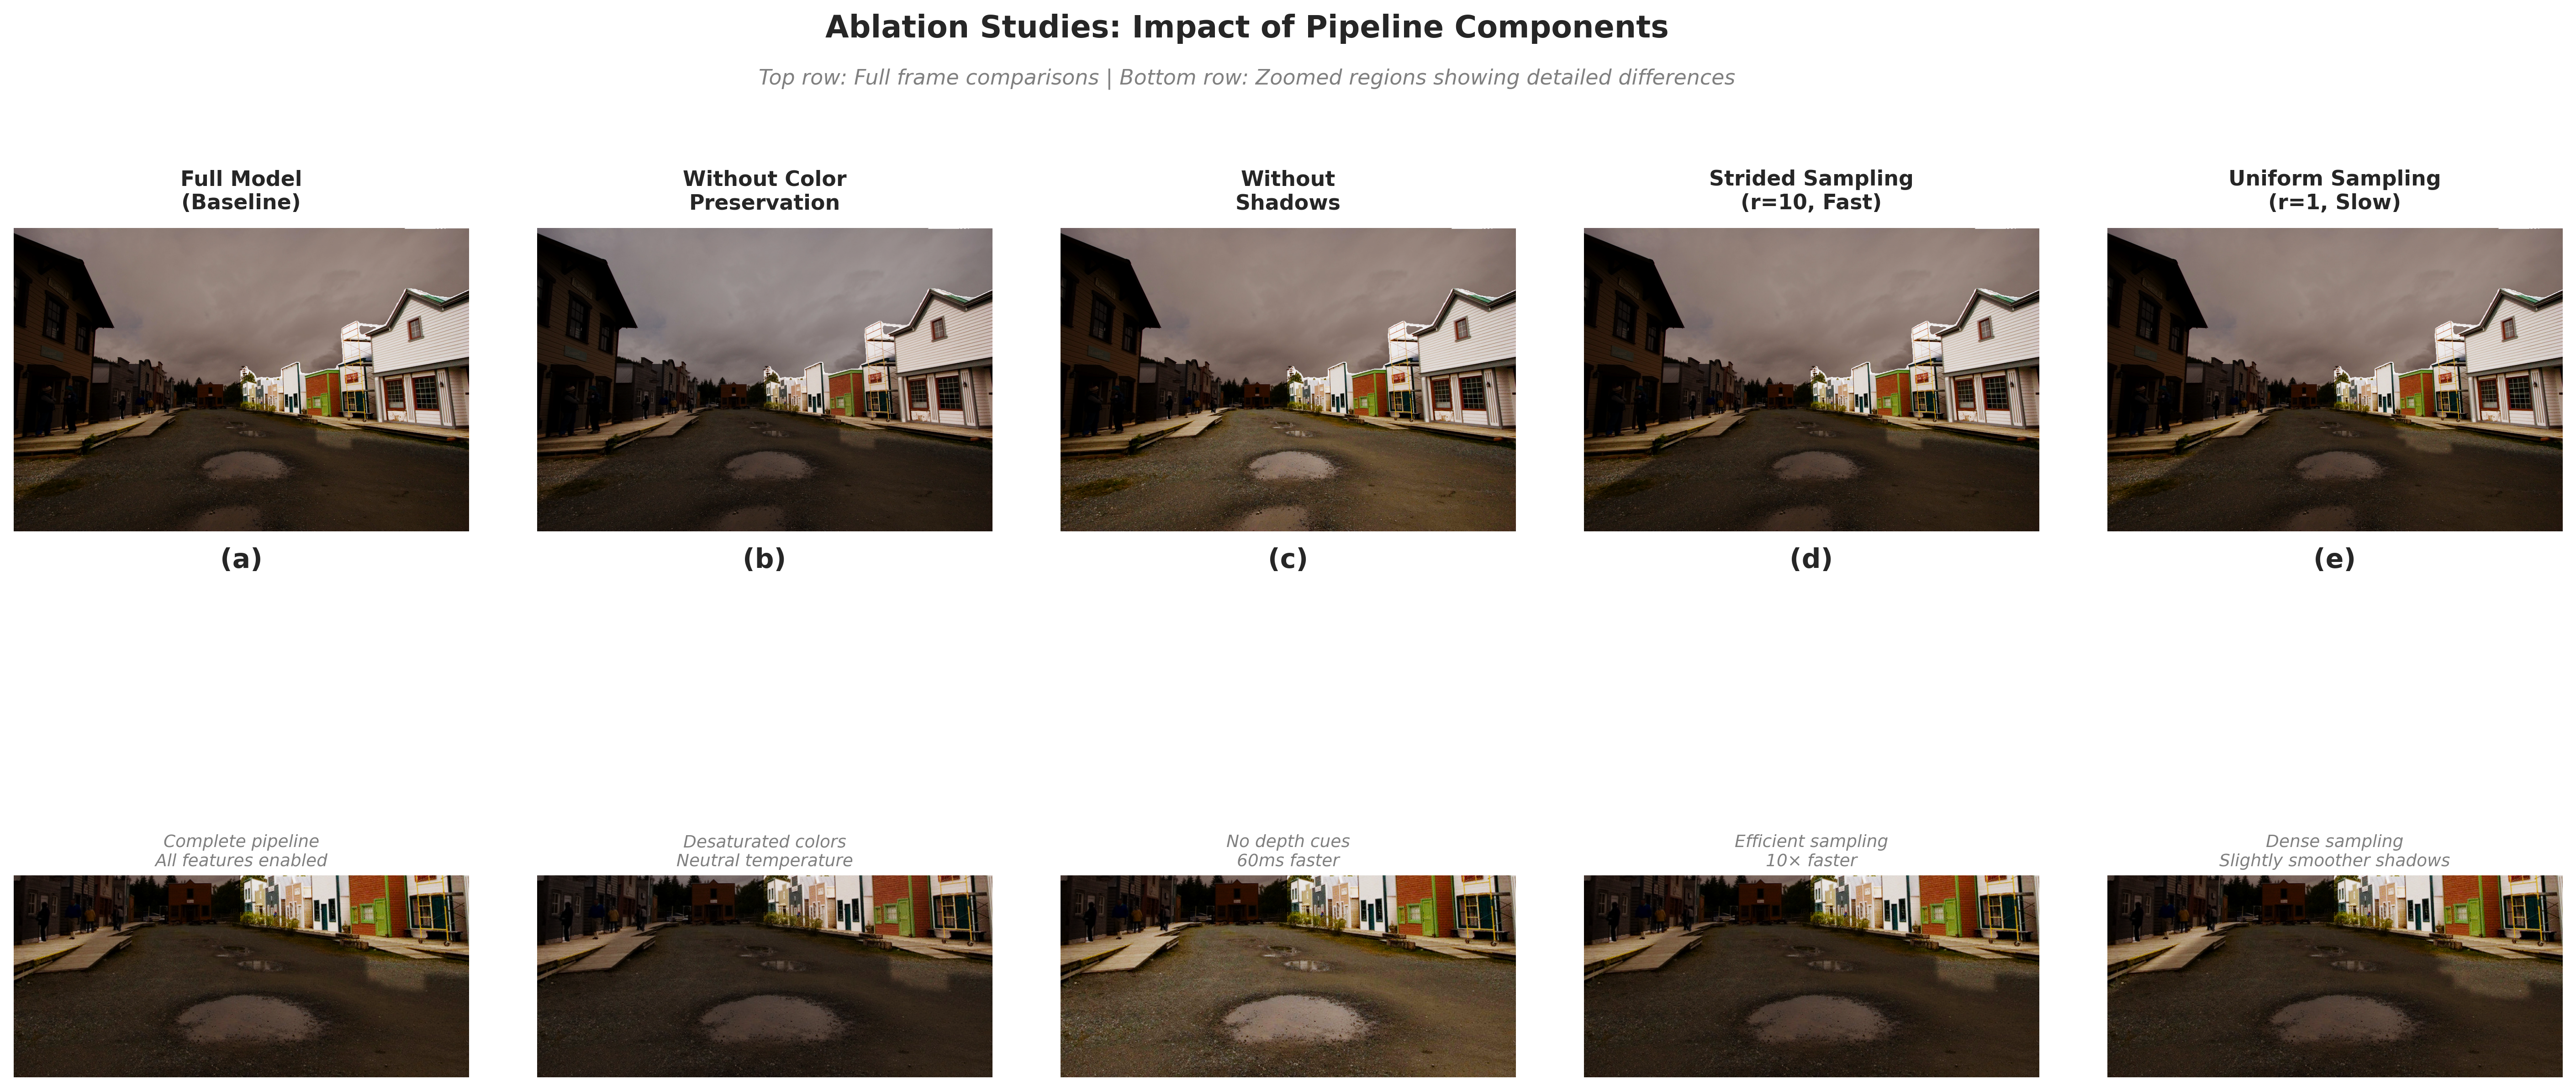
\includegraphics[width=0.8\textwidth]{ablation_studies.png}
    \caption{Impact of key components: (a) Full model (b) No color model (c) No shadows (d) Strided sampling (e) Uniform sampling}
  \end{figure}
  
  \vspace{0.3cm}
  \textbf{Key Findings:}
  \begin{itemize}
    \item Color model essential for realistic appearance
    \item Shadows critical for depth perception (but cost 60ms)
    \item Strided sampling optimal quality-speed tradeoff
  \end{itemize}
\end{frame}

\begin{frame}{System Visualization Gallery}
  \begin{figure}
    \centering
    \includegraphics[width=0.8\textwidth]{visualization_gallery.png}
    \caption{Comprehensive system outputs: 3D trajectories, interactive interface, ray tracing analysis, temporal evolution}
  \end{figure}
  
  \vspace{0.3cm}
  \textbf{Features:}
  \begin{itemize}
    \item Interactive geometry annotation interface
    \item Real-time shadow trajectory visualization
    \item Temporal consistency analysis tools
  \end{itemize}
\end{frame}

\section{Conclusion}

\begin{frame}{Limitations \& Future Work}
  \textbf{Current Limitations:}
  \begin{itemize}
    \item Assumes architectural scenes with single-point perspective
    \item Limited to planar surfaces (shoebox approximation)
    \item Static foreground assumption
    \item No complex geometry or inter-reflections
  \end{itemize}
  
  \vspace{0.5cm}
  \textbf{Future Directions:}
  \begin{itemize}
    \item Extension to multi-point perspective
    \item Learning-based sky-to-geometry refinement
    \item Global illumination via precomputed radiance transfer
    \item Video processing pipeline integration
    \item Support for curved surfaces and complex geometry
  \end{itemize}
\end{frame}

\begin{frame}{Conclusion}
  \textbf{Achievements:}
  \begin{itemize}
    \item \textbf{Practical System:} Single LDR image + sky sequence input
    \item \textbf{Real-Time Performance:} $\sim$150ms/frame on standard CPU
    \item \textbf{High Quality:} Photorealistic results with temporal coherence
    \item \textbf{Accessibility:} No HDR capture or specialized hardware
  \end{itemize}
  
  \vspace{0.5cm}
  \textbf{Technical Contributions:}
  \begin{enumerate}
    \item Interactive SAM-based geometric reconstruction
    \item Efficient LDR sun tracking algorithm
    \item Optimized ray-traced shadow computation
    \item Color-preserving lighting with ACES tone mapping
  \end{enumerate}
  
  \vspace{0.5cm}
  \textbf{Impact:} Democratizes high-quality relighting for everyday photography and time-lapse applications
\end{frame}

\begin{frame}{Demo \& Questions}
  \begin{center}
    \Large
    \textbf{Live Demo}
    
    \vspace{1cm}
    
    % \includegraphics[width=0.6\textwidth]{sky1_results.png}
    % we will add this link
    % https://drive.google.com/file/d/1P7vEAEVtYFdBBX9ZlfudOsBA_YNy8w-5/view
    \vspace{1cm}
    
    \textbf{Questions \& Discussion}
    
    \vspace{0.5cm}
    
    \texttt{shreyas.mehta@students.iiit.ac.in}\\
    \texttt{shubham.goel@students.iiit.ac.in}
  \end{center}
\end{frame}

\end{document}